\PassOptionsToPackage{unicode=true}{hyperref} % options for packages loaded elsewhere
\PassOptionsToPackage{hyphens}{url}
%
\documentclass[]{article}
\usepackage{lmodern}
\usepackage{amssymb,amsmath}
\usepackage{ifxetex,ifluatex}
\usepackage{fixltx2e} % provides \textsubscript
\ifnum 0\ifxetex 1\fi\ifluatex 1\fi=0 % if pdftex
  \usepackage[T1]{fontenc}
  \usepackage[utf8]{inputenc}
  \usepackage{textcomp} % provides euro and other symbols
\else % if luatex or xelatex
  \usepackage{unicode-math}
  \defaultfontfeatures{Ligatures=TeX,Scale=MatchLowercase}
\fi
% use upquote if available, for straight quotes in verbatim environments
\IfFileExists{upquote.sty}{\usepackage{upquote}}{}
% use microtype if available
\IfFileExists{microtype.sty}{%
\usepackage[]{microtype}
\UseMicrotypeSet[protrusion]{basicmath} % disable protrusion for tt fonts
}{}
\IfFileExists{parskip.sty}{%
\usepackage{parskip}
}{% else
\setlength{\parindent}{0pt}
\setlength{\parskip}{6pt plus 2pt minus 1pt}
}
\usepackage{hyperref}
\hypersetup{
            pdftitle={Análisis de expresión RNA-seq para un análisis del tiroides},
            pdfauthor={Marina Ballesteros},
            pdfborder={0 0 0},
            breaklinks=true}
\urlstyle{same}  % don't use monospace font for urls
\usepackage[margin=1in]{geometry}
\usepackage{color}
\usepackage{fancyvrb}
\newcommand{\VerbBar}{|}
\newcommand{\VERB}{\Verb[commandchars=\\\{\}]}
\DefineVerbatimEnvironment{Highlighting}{Verbatim}{commandchars=\\\{\}}
% Add ',fontsize=\small' for more characters per line
\usepackage{framed}
\definecolor{shadecolor}{RGB}{248,248,248}
\newenvironment{Shaded}{\begin{snugshade}}{\end{snugshade}}
\newcommand{\AlertTok}[1]{\textcolor[rgb]{0.94,0.16,0.16}{#1}}
\newcommand{\AnnotationTok}[1]{\textcolor[rgb]{0.56,0.35,0.01}{\textbf{\textit{#1}}}}
\newcommand{\AttributeTok}[1]{\textcolor[rgb]{0.77,0.63,0.00}{#1}}
\newcommand{\BaseNTok}[1]{\textcolor[rgb]{0.00,0.00,0.81}{#1}}
\newcommand{\BuiltInTok}[1]{#1}
\newcommand{\CharTok}[1]{\textcolor[rgb]{0.31,0.60,0.02}{#1}}
\newcommand{\CommentTok}[1]{\textcolor[rgb]{0.56,0.35,0.01}{\textit{#1}}}
\newcommand{\CommentVarTok}[1]{\textcolor[rgb]{0.56,0.35,0.01}{\textbf{\textit{#1}}}}
\newcommand{\ConstantTok}[1]{\textcolor[rgb]{0.00,0.00,0.00}{#1}}
\newcommand{\ControlFlowTok}[1]{\textcolor[rgb]{0.13,0.29,0.53}{\textbf{#1}}}
\newcommand{\DataTypeTok}[1]{\textcolor[rgb]{0.13,0.29,0.53}{#1}}
\newcommand{\DecValTok}[1]{\textcolor[rgb]{0.00,0.00,0.81}{#1}}
\newcommand{\DocumentationTok}[1]{\textcolor[rgb]{0.56,0.35,0.01}{\textbf{\textit{#1}}}}
\newcommand{\ErrorTok}[1]{\textcolor[rgb]{0.64,0.00,0.00}{\textbf{#1}}}
\newcommand{\ExtensionTok}[1]{#1}
\newcommand{\FloatTok}[1]{\textcolor[rgb]{0.00,0.00,0.81}{#1}}
\newcommand{\FunctionTok}[1]{\textcolor[rgb]{0.00,0.00,0.00}{#1}}
\newcommand{\ImportTok}[1]{#1}
\newcommand{\InformationTok}[1]{\textcolor[rgb]{0.56,0.35,0.01}{\textbf{\textit{#1}}}}
\newcommand{\KeywordTok}[1]{\textcolor[rgb]{0.13,0.29,0.53}{\textbf{#1}}}
\newcommand{\NormalTok}[1]{#1}
\newcommand{\OperatorTok}[1]{\textcolor[rgb]{0.81,0.36,0.00}{\textbf{#1}}}
\newcommand{\OtherTok}[1]{\textcolor[rgb]{0.56,0.35,0.01}{#1}}
\newcommand{\PreprocessorTok}[1]{\textcolor[rgb]{0.56,0.35,0.01}{\textit{#1}}}
\newcommand{\RegionMarkerTok}[1]{#1}
\newcommand{\SpecialCharTok}[1]{\textcolor[rgb]{0.00,0.00,0.00}{#1}}
\newcommand{\SpecialStringTok}[1]{\textcolor[rgb]{0.31,0.60,0.02}{#1}}
\newcommand{\StringTok}[1]{\textcolor[rgb]{0.31,0.60,0.02}{#1}}
\newcommand{\VariableTok}[1]{\textcolor[rgb]{0.00,0.00,0.00}{#1}}
\newcommand{\VerbatimStringTok}[1]{\textcolor[rgb]{0.31,0.60,0.02}{#1}}
\newcommand{\WarningTok}[1]{\textcolor[rgb]{0.56,0.35,0.01}{\textbf{\textit{#1}}}}
\usepackage{longtable,booktabs}
% Fix footnotes in tables (requires footnote package)
\IfFileExists{footnote.sty}{\usepackage{footnote}\makesavenoteenv{longtable}}{}
\usepackage{graphicx,grffile}
\makeatletter
\def\maxwidth{\ifdim\Gin@nat@width>\linewidth\linewidth\else\Gin@nat@width\fi}
\def\maxheight{\ifdim\Gin@nat@height>\textheight\textheight\else\Gin@nat@height\fi}
\makeatother
% Scale images if necessary, so that they will not overflow the page
% margins by default, and it is still possible to overwrite the defaults
% using explicit options in \includegraphics[width, height, ...]{}
\setkeys{Gin}{width=\maxwidth,height=\maxheight,keepaspectratio}
\setlength{\emergencystretch}{3em}  % prevent overfull lines
\providecommand{\tightlist}{%
  \setlength{\itemsep}{0pt}\setlength{\parskip}{0pt}}
\setcounter{secnumdepth}{5}
% Redefines (sub)paragraphs to behave more like sections
\ifx\paragraph\undefined\else
\let\oldparagraph\paragraph
\renewcommand{\paragraph}[1]{\oldparagraph{#1}\mbox{}}
\fi
\ifx\subparagraph\undefined\else
\let\oldsubparagraph\subparagraph
\renewcommand{\subparagraph}[1]{\oldsubparagraph{#1}\mbox{}}
\fi

% set default figure placement to htbp
\makeatletter
\def\fps@figure{htbp}
\makeatother

\usepackage{float}

\title{Análisis de expresión RNA-seq para un análisis del tiroides}
\author{Marina Ballesteros}
\date{6/13/2020}

\begin{document}
\maketitle

{
\setcounter{tocdepth}{2}
\tableofcontents
}
\hypertarget{abstract}{%
\section{Abstract}\label{abstract}}

Este análisis se basa en el estudio de expresión de 30 muestras de
RNA-seq pertenecientes al tejido tiroides con el fin de comparar los
tres tipos de infiltración medio: not infiltrated tissues (NIT), small
focal infiltrates (SFI) y extensive lymphoid infiltrates (ELI). Los
datos han sido obtenidos gracias al proyecto The Genotype-Tissue
Expression (GTEx), el cual es una base de datos pública para estudiar la
expresión génica y la regulación de tejidos. En esta fuente de datos se
recogen muestras de 54 tejidos no enfermo en aproximadamente 1000
individuos para llevar a cabo diferentes ensayos moleculares.

Los datos y el código completo del análisis se encuentran en el
siguiente \textbf{repositorio github}
{[}\url{https://github.com/marinabf93/Analisis-Expresion-RNAseq.git}{]}

\hypertarget{objetivos}{%
\section{Objetivos}\label{objetivos}}

Para este análisis he marcado dos objetivos bien diferenciados:

\begin{enumerate}
\def\labelenumi{\alph{enumi})}
\item
  Comparar los tres grupos entre sí e identificar los genes más
  significativos diferencialmente expresados en cada comparación con sus
  correspondientes anotaciones.
\item
  Identificar los procesos biológicos, componentes celulares o funciones
  molesculares más afectados o implicados en el estudio.
\end{enumerate}

\hypertarget{materiales}{%
\section{Materiales}\label{materiales}}

La razón de este trabajo es analizar bioinformáticamente los datos de un
experimento con RNA-seq. Los datos en el que se ha basado el análisis
han sido aportados junto al enunciado de la PEC pero pertenecen al
portal GTEx (\url{https://www.gtexportal.org/home/})
{[}@lonsdale2013genotype{]}

Dentro de los distintos paquetes existentes para el análisis de RNA-seq,
he escogido el \textbf{paquete edgeR} para realizar el análisis
{[}@robinson2010edger{]}. El material en el que he basado todo mi
análisis ha sido la guía de utilización del paquete edgeR: ``edgeR:
differential expression analysis of digital gene expression data''
(\url{http://www.bioconductor.org/packages/release/bioc/vignettes/edgeR/inst/doc/edgeRUsersGuide.pdf})

\hypertarget{diseuxf1o-experimental}{%
\subsection{Diseño experimental}\label{diseuxf1o-experimental}}

El \textbf{tipo de experimento} corresponde al análisis de RNA-seq,
donde a través del diseño de un experimento se intenta responder a los
objetivos planteados. Con el uso de la estadística y las diferentes
herramientas bioinformáticas, se pretende procesar, analizar, visualizar
y analizar los datos con el fin de responder a las cuestiones biológicas
de partida.

El punto de partida de un experimento de ARN-Seq es un conjunto de
muestras de ARN, típicamente asociadas con una variedad de condiciones
de tratamiento. Cada muestra se secuencia, se asignan lecturas cortas al
genoma apropiado y se registra el número de lecturas asignadas a cada
característica genómica de interés. El conjunto de recuentos genéticos
de cada muestra constituye la librería de expresión de esa muestra. El
tamaño esperado de cada recuento es el producto del tamaño de la
librería y la abundancia relativa de ese gen en esa muestra.

El paquete que he elegido ( \textbf{edgeR} ) trabaja en una tabla de
recuentos de lectura de números enteros, con filas correspondientes a
los genes y columnas a las librerías independientes. Los recuentos
representan el número total de lecturas alineadas a cada gen (u otro
locus genómico).Esos recuentos pueden producirse a partir de lecturas
alineadas por una variedad de herramientas de software de lectura corta.

Las lecturas pueden ser contadas de varias maneras. Cuando se realizan
análisis a nivel genético, los conteos podrían ser para mapear lecturas
en cualquier lugar del rango genómico del gen, como en este análisis, o
los conteos podrían ser sólo para exones. Normalmente contamos lecturas
que se superponen a cualquier exón para el gen dado, incluyendo el UTR
como parte del primer exón.

\hypertarget{datos}{%
\subsection{Datos}\label{datos}}

En el caso particular de este análisis se parte directamente de los
\textbf{datos de conteo} en forma de una tabla rectangular de valores
enteros. La celda de la tabla en la fila g-ésima y la columna j-ésima de
la tabla indica cuántas lecturas se han asignado al gen g en la muestra
j.

Además de la tabla con los datos de conteo, se aporta una tabla llamada
\textbf{targets} con toda la información necesaria relativa al estudio:
el ID del experimento, el nombre de las muestras, el grupo al que
pertenecen, el tipo de dato molecular, etc. Ambos datos han sido
aportados por el profesor de la asignatura ``Análisis de datos ómicos''
de la UOC.

\hypertarget{software}{%
\subsection{Software}\label{software}}

Para comenzar el análisis se necesita instalar \textbf{R statistical
software} el cual permite hacer análisis estadísticos, representaciones
gráficas y lectura y creación de documentos en diferentes formatos. El
software se puede descargar en la página web
{[}\url{https://cran.r-project.org/index.html}{]} y solo deben seguirse
las instrucciones indicadas en función del tipo de software del
ordenador que se utilice para el análisis.

El análisis de RNA-seq que se presenta en este informe ha sido
desarrollado con la versión 3.6.2 y todos los análisis se han llevado a
cabo con la interfaz \emph{RStudio}. Esta interfaz puede descargarse
desde la página principal {[}\url{https://www.rstudio.com/}{]}

\hypertarget{muxe9todos-procedimiento-general-del-anuxe1lisis-workflow}{%
\section{Métodos: Procedimiento general del análisis
(``Workflow'')}\label{muxe9todos-procedimiento-general-del-anuxe1lisis-workflow}}

El flujo de trabajo se resumen en la siguiente imagen ``Workflow.png''
dentro del directorio \textbf{figures}.

\begin{figure}[H]

{\centering 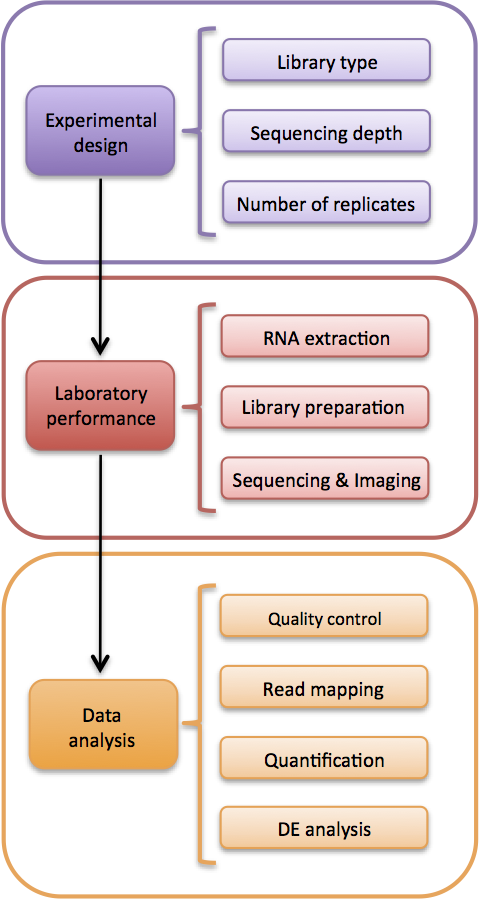
\includegraphics[width=6.65in,]{./figures/Workflow} 

}

\caption{Worflow RNA-seq análisis.}\label{fig:unnamed-chunk-1}
\end{figure}

A continuación resumiré de forma muy general los métodos utilizados en
cada paso del flujo de trabajo. El desarrollo detallado de cada paso del
análisis lo encontraréis en el archivo \textbf{Pipeline del análisis
RNA-seq.Rmd} dentro del directorio principal del repositorio github
indicado al inicio de este informe.

Antes de empezar con el análisis y a manejar la enorme cantidad de datos
y ficheros que ello conlleva, crearé tres carpetas para la organización
del mismo:

\begin{itemize}
\tightlist
\item
  La carpeta principal del análisis será ``Analisis-Expresion-RNAseq'',
  la cual también será mi directorio de trabajo.
\item
  Una carpeta llamada \textbf{data} para almecenar todo tipo de datos
  del experimento y en los cuales basaré mi análisis. En esta carpeta
  guardaré los archivos \emph{counts} y el archivo \emph{targets}, en el
  cual se decribirán los factores de estudio y sus niveles.
\item
  En la carpeta \textbf{results} guardaré todos los resultados obtenidos
  en el análisis.
\item
  La carpeta \textbf{figures} servirá para almacenar todo tipo de
  imágenes y figuras generadas durante el análisis.
\end{itemize}

\hypertarget{definiciuxf3n-de-los-datos}{%
\subsection{Definición de los datos}\label{definiciuxf3n-de-los-datos}}

El primer paso es leer los archivos \textbf{counts.csv} y
\textbf{targets.csv} aportados junto el enunciado de la PEC, ambos
archivos están ubicados en una la carpeta \textbf{data} en el directorio
principal de trabajo.

El archivo \emph{targets.csv} es un resumen de cada experinecia donde
aparecen informaciones como el grupo, sexo o nombre de la muestra. La
columna \emph{group} de este archivo nos informa de los tres grupos de
muestras existentes:

-Not infiltrated tissues (NIT) -Small focal infiltrates (SFI) -Extensive
lymphoid infiltrates (ELI)

El archivo \emph{counts.csv} contiene en sus columnas el nombre de las
292 muestras y cada fila pertenece a un gen diferente.

El siguiente paso fue escoger 30 muestras dentro de las 292 muestras
posibles, de manera que tenga 10 muestras de cada uno de los tres grupos
de tiroides. Para llevar a cabo esto, necesito seleccionar primero 10
muestras de cada grupo a través de la columna \emph{group} del archivo
\textbf{targets.csv}.

\begin{Shaded}
\begin{Highlighting}[]
\KeywordTok{library}\NormalTok{(dplyr)}
\end{Highlighting}
\end{Shaded}

\begin{verbatim}
## 
## Attaching package: 'dplyr'
\end{verbatim}

\begin{verbatim}
## The following objects are masked from 'package:stats':
## 
##     filter, lag
\end{verbatim}

\begin{verbatim}
## The following objects are masked from 'package:base':
## 
##     intersect, setdiff, setequal, union
\end{verbatim}

\begin{Shaded}
\begin{Highlighting}[]
\NormalTok{group_NIT<-}\KeywordTok{subset}\NormalTok{(targets, Group}\OperatorTok{==}\StringTok{"NIT"}\NormalTok{)[}\DecValTok{1}\OperatorTok{:}\DecValTok{10}\NormalTok{,]}
\NormalTok{group_SFI<-}\KeywordTok{subset}\NormalTok{(targets, Group}\OperatorTok{==}\StringTok{"SFI"}\NormalTok{)[}\DecValTok{1}\OperatorTok{:}\DecValTok{10}\NormalTok{,]}
\NormalTok{group_ELI<-}\KeywordTok{subset}\NormalTok{(targets, Group}\OperatorTok{==}\StringTok{"ELI"}\NormalTok{)[}\DecValTok{1}\OperatorTok{:}\DecValTok{10}\NormalTok{,]}

\CommentTok{#Unimos los tres data frame creados en uno solo}
\NormalTok{targets_}\DecValTok{30}\NormalTok{<-}\KeywordTok{Reduce}\NormalTok{(}\ControlFlowTok{function}\NormalTok{(...) }\KeywordTok{merge}\NormalTok{(...,}\DataTypeTok{all=}\OtherTok{TRUE}\NormalTok{), }\KeywordTok{list}\NormalTok{(group_NIT, group_SFI, group_ELI))}
\end{Highlighting}
\end{Shaded}

Una vez he escogido las 30 muestras, extraigo las columnas
correspondientes (en el archivo \textbf{counts.csv}) a esas 30 filas
seleccionadas para finalmente obtener el archivo \textbf{counts\_30}.
Este archivo contiene las 30 muestras con 56202 observaciones (genes) y
será la base de todo el análisis. A continuación se muestran las 5
primeras muestras de este archivo.

\begin{verbatim}
##   GTEX.111CU.0226.SM.5GZXC GTEX.111FC.1026.SM.5GZX1 GTEX.111VG.0526.SM.5N9BW
## 1                        7                        0                        1
## 2                      401                     1064                      474
## 3                        4                        0                        1
## 4                        2                        0                        0
## 5                        0                        0                        1
##   GTEX.111YS.0726.SM.5GZY8 GTEX.1122O.0226.SM.5N9DA GTEX.1128S.0126.SM.5H12S
## 1                        4                        2                        2
## 2                      395                      732                      631
## 3                        2                        1                        0
## 4                        1                        1                        0
## 5                        0                        0                        0
##   GTEX.113JC.0126.SM.5EGJW GTEX.117XS.0526.SM.5987Q GTEX.117YW.0126.SM.5EGGN
## 1                        0                        3                        1
## 2                      331                      511                      483
## 3                        1                        1                        0
## 4                        0                        4                        0
## 5                        0                        0                        0
##   GTEX.117YX.1226.SM.5H11S GTEX.1192W.0126.SM.5EGGS GTEX.1192X.1126.SM.5EGGU
## 1                        3                        3                        2
## 2                      529                      573                      674
## 3                        0                        1                        3
## 4                        1                        0                        1
## 5                        0                        0                        1
##   GTEX.11DXY.0426.SM.5H12R GTEX.11EQ8.0826.SM.5N9FG GTEX.11EQ9.0626.SM.5A5K1
## 1                        0                        1                        6
## 2                      663                      802                      640
## 3                        0                        1                        4
## 4                        0                        0                        3
## 5                        0                        1                        1
##   GTEX.11GS4.0826.SM.5986J GTEX.11NV4.0626.SM.5N9BR GTEX.11O72.2326.SM.5BC7H
## 1                        0                        3                        0
## 2                      533                     1301                      633
## 3                        1                        1                        2
## 4                        1                        0                        1
## 5                        0                        0                        0
##   GTEX.11TUW.0226.SM.5LU8X GTEX.11XUK.0226.SM.5EQLW GTEX.1211K.0726.SM.5FQUW
## 1                        4                        0                        3
## 2                      627                      419                      426
## 3                        0                        0                        1
## 4                        1                        1                        1
## 5                        0                        0                        1
##   GTEX.12584.0826.SM.5FQSK GTEX.12BJ1.0426.SM.5FQSO GTEX.13NZ9.1126.SM.5MR37
## 1                        1                        1                        0
## 2                     1064                      410                     1002
## 3                        2                        2                        1
## 4                        0                        1                        0
## 5                        2                        0                        0
##   GTEX.13QJC.0826.SM.5RQKC GTEX.14ABY.0926.SM.5Q5DY GTEX.14AS3.0226.SM.5Q5B6
## 1                        0                        1                        0
## 2                      825                      775                      834
## 3                        1                        2                        1
## 4                        0                        0                        1
## 5                        0                        0                        0
##   GTEX.14BMU.0226.SM.5S2QA GTEX.PLZ4.1226.SM.2I5FE GTEX.R55G.0726.SM.2TC6J
## 1                        2                       5                       3
## 2                      423                     489                     134
## 3                        0                       1                       1
## 4                        0                       3                       2
## 5                        2                       2                       1
\end{verbatim}

\hypertarget{filtraciuxf3n-de-los-genes}{%
\subsection{Filtración de los genes}\label{filtraciuxf3n-de-los-genes}}

Filtraré los genes reteniendo sólo aquellos genes que se expresen en
todas las muestras y con un número mínimo de contajes. El proceso de
filtraje es muy importante ya que los genes con recuentos muy bajos en
las librerías no proporcionan apenas pruebas de expresión diferencial y,
además, interfieren de forma negativa en algunas aproximaciones
estadísticas. En consecuecia, estos genes con bajos conteos reducen el
poder de detección de los genes de expresión diferencial y por ello es
importante eliminarlos. Para llevar a cabo el filtraje necesito primero
descargar el paquete \textbf{edgeR} de Bioconductor.

Hay distintas formas de filtrar los genes de baja expresión pero antes
se deben transformar los conteos con el fin de tener en una misma escala
todas las muestras de un mismo estudio y evitar, así, diferencias debido
al distinto tamaño de las librerías.

En este estudio por cada grupo existen 10 réplicas biológicas, ya que el
tamaño de muestra de cada grupo es 10. Por este motivo, estableceré un
umbral mínimo de conteos por millón (CPM) en al menos 10 muestras; es
decir, favoreceré un filtraje donde los genes estén representados al
menos una vez en todas las muestras en cada grupo.

El segundo umbral que puedo marcar para el filtraje es un mínimo de
conteos por millón para cada gen. Para obtener el número de conteos por
millón utilizaré la función \textbf{cpm} del paquete \emph{edgeR}. Esta
función permite convertir los contajes a CPMs, por lo tanto, se están
normalizando los conteos para las diferentes profundidades de
secuenciación de cada muestra.

Por regla general, se puede elegir un buen umbral mínimo de CPMs
identificando el CPM que corresponde a un conteo de 10. Contrastando las
tablas \textbf{counts\_30} y \textbf{myCPM}, se observa que el umbral en
este caso es aproximadamente 0,15. Con la selección de genes que superen
el umbral de 0,15 se obtiene una matriz lógica con los genes que han
superado el umbral (TRUE) y los genes que estan por debajo del umbral
(FALSE). Se muestran los resultados de los tres primeros genes para la
superación o no de dicho umbral.

\begin{Shaded}
\begin{Highlighting}[]
\NormalTok{knitr}\OperatorTok{::}\KeywordTok{kable}\NormalTok{(}
\NormalTok{  table1, }\DataTypeTok{booktabs =} \OtherTok{TRUE}\NormalTok{,}
  \DataTypeTok{caption =} \StringTok{'Matriz lógica donde se recogen como TRUE los genes que superan CPM > 0.15 y como FALSE los genes que no superan dicho umbral.'}\NormalTok{)}
\end{Highlighting}
\end{Shaded}

\begin{longtable}[]{@{}llllllllllllllllllllllllllllll@{}}
\caption{Matriz lógica donde se recogen como TRUE los genes que superan
CPM \textgreater{} 0.15 y como FALSE los genes que no superan dicho
umbral.}\tabularnewline
\toprule
GTEX.111CU.0226.SM.5GZXC & GTEX.111FC.1026.SM.5GZX1 &
GTEX.111VG.0526.SM.5N9BW & GTEX.111YS.0726.SM.5GZY8 &
GTEX.1122O.0226.SM.5N9DA & GTEX.1128S.0126.SM.5H12S &
GTEX.113JC.0126.SM.5EGJW & GTEX.117XS.0526.SM.5987Q &
GTEX.117YW.0126.SM.5EGGN & GTEX.117YX.1226.SM.5H11S &
GTEX.1192W.0126.SM.5EGGS & GTEX.1192X.1126.SM.5EGGU &
GTEX.11DXY.0426.SM.5H12R & GTEX.11EQ8.0826.SM.5N9FG &
GTEX.11EQ9.0626.SM.5A5K1 & GTEX.11GS4.0826.SM.5986J &
GTEX.11NV4.0626.SM.5N9BR & GTEX.11O72.2326.SM.5BC7H &
GTEX.11TUW.0226.SM.5LU8X & GTEX.11XUK.0226.SM.5EQLW &
GTEX.1211K.0726.SM.5FQUW & GTEX.12584.0826.SM.5FQSK &
GTEX.12BJ1.0426.SM.5FQSO & GTEX.13NZ9.1126.SM.5MR37 &
GTEX.13QJC.0826.SM.5RQKC & GTEX.14ABY.0926.SM.5Q5DY &
GTEX.14AS3.0226.SM.5Q5B6 & GTEX.14BMU.0226.SM.5S2QA &
GTEX.PLZ4.1226.SM.2I5FE & GTEX.R55G.0726.SM.2TC6J\tabularnewline
\midrule
\endfirsthead
\toprule
GTEX.111CU.0226.SM.5GZXC & GTEX.111FC.1026.SM.5GZX1 &
GTEX.111VG.0526.SM.5N9BW & GTEX.111YS.0726.SM.5GZY8 &
GTEX.1122O.0226.SM.5N9DA & GTEX.1128S.0126.SM.5H12S &
GTEX.113JC.0126.SM.5EGJW & GTEX.117XS.0526.SM.5987Q &
GTEX.117YW.0126.SM.5EGGN & GTEX.117YX.1226.SM.5H11S &
GTEX.1192W.0126.SM.5EGGS & GTEX.1192X.1126.SM.5EGGU &
GTEX.11DXY.0426.SM.5H12R & GTEX.11EQ8.0826.SM.5N9FG &
GTEX.11EQ9.0626.SM.5A5K1 & GTEX.11GS4.0826.SM.5986J &
GTEX.11NV4.0626.SM.5N9BR & GTEX.11O72.2326.SM.5BC7H &
GTEX.11TUW.0226.SM.5LU8X & GTEX.11XUK.0226.SM.5EQLW &
GTEX.1211K.0726.SM.5FQUW & GTEX.12584.0826.SM.5FQSK &
GTEX.12BJ1.0426.SM.5FQSO & GTEX.13NZ9.1126.SM.5MR37 &
GTEX.13QJC.0826.SM.5RQKC & GTEX.14ABY.0926.SM.5Q5DY &
GTEX.14AS3.0226.SM.5Q5B6 & GTEX.14BMU.0226.SM.5S2QA &
GTEX.PLZ4.1226.SM.2I5FE & GTEX.R55G.0726.SM.2TC6J\tabularnewline
\midrule
\endhead
FALSE & FALSE & FALSE & FALSE & FALSE & FALSE & FALSE & FALSE & FALSE &
FALSE & FALSE & FALSE & FALSE & FALSE & FALSE & FALSE & FALSE & FALSE &
FALSE & FALSE & FALSE & FALSE & FALSE & FALSE & FALSE & FALSE & FALSE &
FALSE & FALSE & TRUE\tabularnewline
TRUE & TRUE & TRUE & TRUE & TRUE & TRUE & TRUE & TRUE & TRUE & TRUE &
TRUE & TRUE & TRUE & TRUE & TRUE & TRUE & TRUE & TRUE & TRUE & TRUE &
TRUE & TRUE & TRUE & TRUE & TRUE & TRUE & TRUE & TRUE & TRUE &
TRUE\tabularnewline
FALSE & FALSE & FALSE & FALSE & FALSE & FALSE & FALSE & FALSE & FALSE &
FALSE & FALSE & FALSE & FALSE & FALSE & FALSE & FALSE & FALSE & FALSE &
FALSE & FALSE & FALSE & FALSE & FALSE & FALSE & FALSE & FALSE & FALSE &
FALSE & FALSE & FALSE\tabularnewline
\bottomrule
\end{longtable}

Una vez he filtrado los genes, hago un resumen con los genes que tienen
un valor CPM superior al valor umbral. Dentro de los genes seleccionados
como \emph{TRUE}, seleccionaré los genes que tienen al menos 10 valores
TRUE para cada gen; es decir, me quedaré con los genes que tengan
representación en todas las muestras del grupo.

Los genes que superen los dos umbrales se seleccionan y recogen en el
objeto \emph{counts.keep} y estos serán los únicos conteos que
conservaré para posteriores análisis. En este caso partimos de 56202
genes y tan solo conservaré 22990 genes tras la filtración.

\begin{verbatim}
##    Mode   FALSE    TRUE 
## logical   33212   22990
\end{verbatim}

\begin{verbatim}
## [1] 22990    30
\end{verbatim}

Hasta aquí llega el proceso de filtraje, ahora debo convertir los
conteos en un objeto de la clase \textbf{DEGList}; este objeto es propio
del paquete \emph{edgeR} y sirve para almacenar datos de conteos con los
parámetros que se consideren pertinentes. En este caso sólo añadiré como
parámetro la clasificación de las muestras en el grupo correspondiente
gracias al objeto \emph{group} creado junto con la tabla de conteos
\emph{counts\_30}. El objeto \emph{group} me permite identificar el
grupo al que pertenece cada muestra tal y como se muestra en la
siguiente tabla.

\begin{Shaded}
\begin{Highlighting}[]
\NormalTok{knitr}\OperatorTok{::}\KeywordTok{kable}\NormalTok{(}
\NormalTok{  y}\OperatorTok{$}\NormalTok{samples, }\DataTypeTok{booktabs =} \OtherTok{TRUE}\NormalTok{,}
  \DataTypeTok{caption =} \StringTok{'Tabla del objeto DGEList donde para cada muestra se incluye el grupo, el tamaño de la librería y el factor de normalización.'}\NormalTok{)}
\end{Highlighting}
\end{Shaded}

\begin{longtable}[]{@{}llrr@{}}
\caption{Tabla del objeto DGEList donde para cada muestra se incluye el
grupo, el tamaño de la librería y el factor de
normalización.}\tabularnewline
\toprule
& group & lib.size & norm.factors\tabularnewline
\midrule
\endfirsthead
\toprule
& group & lib.size & norm.factors\tabularnewline
\midrule
\endhead
GTEX.111CU.0226.SM.5GZXC & NIT & 66132137 & 1\tabularnewline
GTEX.111FC.1026.SM.5GZX1 & NIT & 55915131 & 1\tabularnewline
GTEX.111VG.0526.SM.5N9BW & ELI & 52167486 & 1\tabularnewline
GTEX.111YS.0726.SM.5GZY8 & NIT & 48970410 & 1\tabularnewline
GTEX.1122O.0226.SM.5N9DA & NIT & 53818958 & 1\tabularnewline
GTEX.1128S.0126.SM.5H12S & NIT & 47477039 & 1\tabularnewline
GTEX.113JC.0126.SM.5EGJW & NIT & 50137659 & 1\tabularnewline
GTEX.117XS.0526.SM.5987Q & NIT & 41440706 & 1\tabularnewline
GTEX.117YW.0126.SM.5EGGN & SFI & 37403355 & 1\tabularnewline
GTEX.117YX.1226.SM.5H11S & NIT & 52045327 & 1\tabularnewline
GTEX.1192W.0126.SM.5EGGS & NIT & 43547734 & 1\tabularnewline
GTEX.1192X.1126.SM.5EGGU & NIT & 43035398 & 1\tabularnewline
GTEX.11DXY.0426.SM.5H12R & SFI & 53058256 & 1\tabularnewline
GTEX.11EQ8.0826.SM.5N9FG & SFI & 55742090 & 1\tabularnewline
GTEX.11EQ9.0626.SM.5A5K1 & SFI & 73420195 & 1\tabularnewline
GTEX.11GS4.0826.SM.5986J & SFI & 50356711 & 1\tabularnewline
GTEX.11NV4.0626.SM.5N9BR & ELI & 51917213 & 1\tabularnewline
GTEX.11O72.2326.SM.5BC7H & SFI & 68463803 & 1\tabularnewline
GTEX.11TUW.0226.SM.5LU8X & SFI & 44913853 & 1\tabularnewline
GTEX.11XUK.0226.SM.5EQLW & ELI & 49964100 & 1\tabularnewline
GTEX.1211K.0726.SM.5FQUW & SFI & 51857837 & 1\tabularnewline
GTEX.12584.0826.SM.5FQSK & SFI & 51981678 & 1\tabularnewline
GTEX.12BJ1.0426.SM.5FQSO & SFI & 54105277 & 1\tabularnewline
GTEX.13NZ9.1126.SM.5MR37 & ELI & 61398921 & 1\tabularnewline
GTEX.13QJC.0826.SM.5RQKC & ELI & 48806596 & 1\tabularnewline
GTEX.14ABY.0926.SM.5Q5DY & ELI & 64676809 & 1\tabularnewline
GTEX.14AS3.0226.SM.5Q5B6 & ELI & 41984061 & 1\tabularnewline
GTEX.14BMU.0226.SM.5S2QA & ELI & 44456272 & 1\tabularnewline
GTEX.PLZ4.1226.SM.2I5FE & ELI & 64405789 & 1\tabularnewline
GTEX.R55G.0726.SM.2TC6J & ELI & 15468340 & 1\tabularnewline
\bottomrule
\end{longtable}

\hypertarget{control-de-calidad-de-los-datos-filtrados}{%
\subsection{Control de calidad de los datos
filtrados}\label{control-de-calidad-de-los-datos-filtrados}}

El objetivo del control de calidad es revelar posibles problemas
técnicos u otros sesgos presentes en los datos. La mejor manera para
llevar a cabo un control de calidad es de manera visual. El primer paso,
por lo tanto, será representar los datos gráficamente.

El primer gráfico será una representación de los tamaños de las
distintas librerías con un gráfico de barras para ver si hay grandes
discrepancias entre las muestras.

\begin{figure}[H]

{\centering \includegraphics{Informe-del-análisis_files/figure-latex/unnamed-chunk-2-1} 

}

\caption{Barplot que representa el tamaño de las librerías de cada muestra.}\label{fig:unnamed-chunk-2}
\end{figure}

En el gráfico se aprecia que las dimensiones de las librerías varían
entre 15 y 70 millones de conteos. Estas enormes diferencias en el
tamaño de las librerías indica que una normalización de los datos es
necesaria antes de llevar a cabo los análisis de expresión diferencial.

Los datos de conteo no están distribuidos normalmente, así que si quiero
examinar las distribuciones de los conteos en bruto necesito convertir
los conteos en logaritmos. Una vez los conteos estén trnaformados en
logaritmos, usaré gráficos de caja para comprobar la distribución de los
recuentos leídos en la escala log2.

\begin{figure}[H]

{\centering \includegraphics{Informe-del-análisis_files/figure-latex/unnamed-chunk-3-1} 

}

\caption{Boxplot de las dsitribuciones de las librerías.}\label{fig:unnamed-chunk-3}
\end{figure}

De las 30 cajas, se observa que en general las distribuciones de
densidad de las intensidades logarítmicas brutas no son idénticas pero
aún así no muy diferentes. Si una muestra está realmente muy por encima
o por debajo de la línea horizontal azul, se necesitaría entonces
investigar esa muestra más a fondo. Los puntos dibujados más allá de los
extremos de las cajas corresponden a valores outliers.

El siguiente gráfico que llevaré a cabo en este control de calidad
visual es un \textbf{Mapa de color}. Este tipo de gráficos sirven para
agrupar las muestras en base a algún método jerárquico. Por lo tanto,
las muestras que se encuentren juntas serán las muestras más similares
entre sí.

\begin{verbatim}
## Loading required package: mixOmics
\end{verbatim}

\begin{verbatim}
## Warning: package 'mixOmics' was built under R version 3.6.3
\end{verbatim}

\begin{verbatim}
## Loading required package: MASS
\end{verbatim}

\begin{verbatim}
## 
## Attaching package: 'MASS'
\end{verbatim}

\begin{verbatim}
## The following object is masked from 'package:dplyr':
## 
##     select
\end{verbatim}

\begin{verbatim}
## Loading required package: lattice
\end{verbatim}

\begin{verbatim}
## Loading required package: ggplot2
\end{verbatim}

\begin{verbatim}
## 
## Loaded mixOmics 6.10.9
## Thank you for using mixOmics!
## Tutorials: http://mixomics.org
## Bookdown vignette: https://mixomicsteam.github.io/Bookdown
## Questions, issues: Follow the prompts at http://mixomics.org/contact-us
## Cite us:  citation('mixOmics')
\end{verbatim}

\begin{verbatim}
## Loading required package: RColorBrewer
\end{verbatim}

\begin{verbatim}
## Error in cim plot: figure margins too large. See ?cim for help.
\end{verbatim}

En el \emph{Heatmap} no existe una clara agrupación entre los tres
grupos, el grupo que más agrupado se encuentra es el \emph{ELI} en la
parte inferior del eje Y. Por el contrario, las muestras de los grupos
\emph{SFI} y \emph{NIT} están entremezcladas. Según la escala de
colores, el color azul representaría los genes que no han cambiado su
expresión ; mientras que el color verde representa los genes que si han
aumentado su expresión. Esto me hace indicar que en la inmensa mayoría
de los casos, los genes de las diferentes muestras han sufrido un
aumento en su expresión, veré si esta predicción se corresponde más
adelante con el análisis de expresión diferencial.

Para acabar con este control de calidad visual, representaré un
\textbf{Plot de componentes principales (PCA)}. Este tipo de gráficos es
útil para visualizar el efecto global de las covariables experimentales
y los efectos de los lotes. En este análisis, el plot PCA agrupa las
muestras por grupos de genes que más significativamente han cambiado su
expresión. Debido a que en este estudio existe un único factor con tres
niveles: SFI, NIT y ELI; debería haber una clara separación de las
muestras en función de estos tres niveles.

\begin{verbatim}
## Loading required package: DESeq
\end{verbatim}

\begin{verbatim}
## Loading required package: BiocGenerics
\end{verbatim}

\begin{verbatim}
## Loading required package: parallel
\end{verbatim}

\begin{verbatim}
## 
## Attaching package: 'BiocGenerics'
\end{verbatim}

\begin{verbatim}
## The following objects are masked from 'package:parallel':
## 
##     clusterApply, clusterApplyLB, clusterCall, clusterEvalQ,
##     clusterExport, clusterMap, parApply, parCapply, parLapply,
##     parLapplyLB, parRapply, parSapply, parSapplyLB
\end{verbatim}

\begin{verbatim}
## The following objects are masked from 'package:dplyr':
## 
##     combine, intersect, setdiff, union
\end{verbatim}

\begin{verbatim}
## The following object is masked from 'package:limma':
## 
##     plotMA
\end{verbatim}

\begin{verbatim}
## The following objects are masked from 'package:float':
## 
##     colnames, rownames, which.max, which.min
\end{verbatim}

\begin{verbatim}
## The following objects are masked from 'package:stats':
## 
##     IQR, mad, sd, var, xtabs
\end{verbatim}

\begin{verbatim}
## The following objects are masked from 'package:base':
## 
##     anyDuplicated, append, as.data.frame, basename, cbind, colnames,
##     dirname, do.call, duplicated, eval, evalq, Filter, Find, get, grep,
##     grepl, intersect, is.unsorted, lapply, Map, mapply, match, mget,
##     order, paste, pmax, pmax.int, pmin, pmin.int, Position, rank,
##     rbind, Reduce, rownames, sapply, setdiff, sort, table, tapply,
##     union, unique, unsplit, which, which.max, which.min
\end{verbatim}

\begin{verbatim}
## Loading required package: Biobase
\end{verbatim}

\begin{verbatim}
## Welcome to Bioconductor
## 
##     Vignettes contain introductory material; view with
##     'browseVignettes()'. To cite Bioconductor, see
##     'citation("Biobase")', and for packages 'citation("pkgname")'.
\end{verbatim}

\begin{verbatim}
## Loading required package: locfit
\end{verbatim}

\begin{verbatim}
## locfit 1.5-9.4    2020-03-24
\end{verbatim}

\begin{verbatim}
##     Welcome to 'DESeq'. For improved performance, usability and
##     functionality, please consider migrating to 'DESeq2'.
\end{verbatim}

\begin{figure}[H]

{\centering \includegraphics{Informe-del-análisis_files/figure-latex/unnamed-chunk-5-1} 

}

\caption{Plot PCA para el análisis de componentes principales}\label{fig:unnamed-chunk-5}
\end{figure}

En el gráfico de \textbf{análisis de componentes principales} se ve una
clara separación de los tres grupos: las muestras pertenecientes al gruo
\emph{ELI} se sitúan a la derecha del gráfico, las muestras del grupo
\emph{SFI} están en la mitad baja del gráfico y, las muestras \emph{NIT}
se ubican en la parte derecha del plot. Sin embargo, se pueden observar
dos muestras que no están situadas con su grupo: una muestra \emph{SFI}
y una muestra \emph{ELI} se sitúan junto a las muestras del grupo
\emph{NIT}. Debido a que son sólo dos muestras, una de cada grupo, no
hablaría de efectos de lote personalmente.

\hypertarget{normalizaciuxf3n-de-los-datos}{%
\subsection{Normalización de los
datos}\label{normalizaciuxf3n-de-los-datos}}

Por último, procedo a la \textbf{normalización} de los datos filtrados.
El paquete \textbf{edgeR} se ocupa del análisis de la expresión
diferencial más que de la cuantificación de los niveles de expresión. Es
decir, se ocupa de los cambios relativos en los niveles de expresión
entre las condiciones. Por esta razón, los problemas de normalización se
plantean sólo en la medida en que los factores técnicos tienen efectos
específicos en la muestra.

Hay dos factores técnicos que pueden afectar a los recuentos de lectura
de expresión diferencial:

\textbf{La profundidad de secuenciación de cada muestra de ARN}. El
paquete \emph{edgeR} ajusta automáticamente cualquier análisis de
expresión diferencial para variar las profundidades de secuenciación,
representadas por diferentes tamaños de librería. \textbf{La producción
total de ARN por célula}. Esto suele ser importante cuando un pequeño
número de genes se expresan en gran medida en una muestra, pero no en
otra. Este efecto provoca que los genes altamente expresados consuman
una proporción sustancial del tamaño total de la librería, lo que hace
que los genes restantes no estén suficientemente muestreados en esa
muestra.

Como el primer factor se corrige automáticamente con el paquete
\emph{edgeR}, debo corregir el segundo factor a través de la función
\textbf{calcNormFactors}. Esta función encontrará un conjunto de
factores de escala para los tamaños de las bibliotecas con el fin de
minimizar los cambios de pliege entre las muestras para la mayoría de
genes. El método por defecto para calcular estos factores de escala
utiliza una media recortada de valores M (TMM) entre cada par de
muestras. La multiplicación del tamaño original de la librería por el
factor de escala se llamará el \textbf{tamaño efectivo de la librería},
que sustituye al tamaño original de la librería en todos los análisis.

En este caso he usadi el método por defecto, Trimmed Mean of M-values
(TMM); ya que observando un poco los datos del archivo \emph{counts\_30}
se ve que el recuento total de lecturas depende en gran medida de unas
pocas transcripciones altamente expresadas.

\begin{Shaded}
\begin{Highlighting}[]
\NormalTok{knitr}\OperatorTok{::}\KeywordTok{kable}\NormalTok{(}
\NormalTok{  y}\OperatorTok{$}\NormalTok{samples, }\DataTypeTok{booktabs =} \OtherTok{TRUE}\NormalTok{,}
  \DataTypeTok{caption =} \StringTok{'Tabla del objeto DGEList tras el proceso de normalización.'}\NormalTok{)}
\end{Highlighting}
\end{Shaded}

\begin{longtable}[]{@{}llrr@{}}
\caption{Tabla del objeto DGEList tras el proceso de
normalización.}\tabularnewline
\toprule
& group & lib.size & norm.factors\tabularnewline
\midrule
\endfirsthead
\toprule
& group & lib.size & norm.factors\tabularnewline
\midrule
\endhead
GTEX.111CU.0226.SM.5GZXC & NIT & 66132137 & 0.8822941\tabularnewline
GTEX.111FC.1026.SM.5GZX1 & NIT & 55915131 & 1.0484240\tabularnewline
GTEX.111VG.0526.SM.5N9BW & ELI & 52167486 & 0.9654989\tabularnewline
GTEX.111YS.0726.SM.5GZY8 & NIT & 48970410 & 0.9651440\tabularnewline
GTEX.1122O.0226.SM.5N9DA & NIT & 53818958 & 0.8689757\tabularnewline
GTEX.1128S.0126.SM.5H12S & NIT & 47477039 & 1.0289663\tabularnewline
GTEX.113JC.0126.SM.5EGJW & NIT & 50137659 & 0.8861010\tabularnewline
GTEX.117XS.0526.SM.5987Q & NIT & 41440706 & 1.0196200\tabularnewline
GTEX.117YW.0126.SM.5EGGN & SFI & 37403355 & 1.0377109\tabularnewline
GTEX.117YX.1226.SM.5H11S & NIT & 52045327 & 0.9629562\tabularnewline
GTEX.1192W.0126.SM.5EGGS & NIT & 43547734 & 1.1006338\tabularnewline
GTEX.1192X.1126.SM.5EGGU & NIT & 43035398 & 1.0297697\tabularnewline
GTEX.11DXY.0426.SM.5H12R & SFI & 53058256 & 1.0360441\tabularnewline
GTEX.11EQ8.0826.SM.5N9FG & SFI & 55742090 & 1.0359237\tabularnewline
GTEX.11EQ9.0626.SM.5A5K1 & SFI & 73420195 & 0.9274279\tabularnewline
GTEX.11GS4.0826.SM.5986J & SFI & 50356711 & 1.0094869\tabularnewline
GTEX.11NV4.0626.SM.5N9BR & ELI & 51917213 & 1.1269897\tabularnewline
GTEX.11O72.2326.SM.5BC7H & SFI & 68463803 & 0.8734407\tabularnewline
GTEX.11TUW.0226.SM.5LU8X & SFI & 44913853 & 0.9799702\tabularnewline
GTEX.11XUK.0226.SM.5EQLW & ELI & 49964100 & 0.9998036\tabularnewline
GTEX.1211K.0726.SM.5FQUW & SFI & 51857837 & 0.9045863\tabularnewline
GTEX.12584.0826.SM.5FQSK & SFI & 51981678 & 1.0356130\tabularnewline
GTEX.12BJ1.0426.SM.5FQSO & SFI & 54105277 & 0.8834430\tabularnewline
GTEX.13NZ9.1126.SM.5MR37 & ELI & 61398921 & 1.1560360\tabularnewline
GTEX.13QJC.0826.SM.5RQKC & ELI & 48806596 & 1.0291883\tabularnewline
GTEX.14ABY.0926.SM.5Q5DY & ELI & 64676809 & 1.0313566\tabularnewline
GTEX.14AS3.0226.SM.5Q5B6 & ELI & 41984061 & 1.1304005\tabularnewline
GTEX.14BMU.0226.SM.5S2QA & ELI & 44456272 & 1.0074671\tabularnewline
GTEX.PLZ4.1226.SM.2I5FE & ELI & 64405789 & 1.0387770\tabularnewline
GTEX.R55G.0726.SM.2TC6J & ELI & 15468340 & 1.0890683\tabularnewline
\bottomrule
\end{longtable}

Puede observarse que los factores de normalización han cambiado tras la
normalización. Un factor de normalización inferior a uno indica que un
pequeño número de genes de alto recuento monopoliza la secuencia, lo que
hace que los recuentos de otros genes sean inferiores a lo que sería
habitual dado el tamaño de la librería. Como resultado, el tamaño de la
librería se reducirá, de forma análoga a la escalada de los recuentos al
alza en esa librería. Por el contrario, un factor superior a uno aumenta
el tamaño de la librería y equivale a reducir los recuentos.

El rendimiento del procedimiento de normalización de la TMM puede
examinarse mediante gráficos de diferencia media o \textbf{plot MD}.
Estos gráficos muestran la expresión media (media: eje x) frente a los
cambios de logaritmo (diferencia: eje y). Para visulaizar la diferencia
de los gráficos antes y después de la normalización, he generado cuatro
\textbf{plots MD} donde se representan las muestras
\emph{GTEX.111CU.0226.SM.5GZXC} y \emph{GTEX.13NZ9.1126.SM.5MR37}, dos
plots para cada muestra. He elegido la librería de la muestra
\emph{GTEX.111CU.0226.SM.5GZXC} porque es una de las muestras con el
factor de normalización más pequeño: 0.882. Para tener el ejemplo
contrario, he representado igualmente la muestra
\emph{GTEX.13NZ9.1126.SM.5MR37} la cual tiene uno de los factores de
normalización más elevados: 1.156.

Estos son los gráficos de ambas muestras \textbf{antes} de la
normalización.

\begin{figure}[H]

{\centering \includegraphics{Informe-del-análisis_files/figure-latex/unnamed-chunk-6-1} 

}

\caption{Plot MD para el logaritmo de los conteos, normalizados sólo para el tamaño de las librerías.}\label{fig:unnamed-chunk-6}
\end{figure}

En ambos casos se ve con claridad que los valores no se sitúan en torno
a un cambio de pliegue de cero marcado por la línea roja; sino que las
muestras están por debajo y por encima de un cambio de pliegeue de cero
respectivamente.

Sin embargo, en los siguientes \emph{plot MD} se aprecia que el grueso
de genes para ambas muestras se sitúan en torno a un cambio de pliege en
torno a cero, por lo que el sesgo se ha corregido con la normalización
del \emph{objeto y}.

\begin{figure}[H]

{\centering \includegraphics{Informe-del-análisis_files/figure-latex/unnamed-chunk-7-1} 

}

\caption{Plot MD para el objeto y, normalizado tanto para el tamaño de las librerías como para el sesgo de composición.}\label{fig:unnamed-chunk-7}
\end{figure}

Otro gráfico que se suele representar tras la normalización de los
datos, es un \textbf{plot MDS} donde se representan las similitudes
relativas de las 30 muestras en función del tipo de infiltración
existente en el tiroides. Las similitudes se cuantifican en forma de
cambios de pliegue (log folg change) entre muestras.

En el \emph{plot MDS} la primera dimensión representa la magnitud del
cambio biológico que mejor separa las muestras y, por lo tanto, el
cambio biológico que representa la mayor proporción de variación de los
datos.

\begin{figure}[H]

{\centering \includegraphics{Informe-del-análisis_files/figure-latex/unnamed-chunk-8-1} 

}

\caption{Plot MDS para el análisis de distancias entre muestras}\label{fig:unnamed-chunk-8}
\end{figure}

Existe una clara agrupación entre los tres grupos, lo que muestra un
efecto según el tipo de infiltración. Esta tendencia era de esperar
puesto que en este análisis es el único factor a tener en cuenta y
puesto que el plotMDS es un plot muy similar al plot PCA, donde ya se
obtuvieron los mismos resultados.

\hypertarget{identificaciuxf3n-de-genes-diferencialmente-expresados}{%
\subsection{Identificación de genes diferencialmente
expresados}\label{identificaciuxf3n-de-genes-diferencialmente-expresados}}

\hypertarget{matriz-de-diseuxf1o}{%
\subsubsection{Matriz de diseño}\label{matriz-de-diseuxf1o}}

La matriz de diseño contiene los predictores para cada muestra; en la
matriz se asigna un coeficiente a cada grupo. La matriz de diseño se
crea a partir del \emph{objeto y} ya que contiene la información sobre
el grupo experimental al que pertenece cada muestra. En este análisis,
lo interesante son las diferencias entre los tres tipos de infiltración.
Por lo tanto, creo una matriz de diseño utilizando el factor \emph{tipo
de infiltración}.

\begin{Shaded}
\begin{Highlighting}[]
\NormalTok{knitr}\OperatorTok{::}\KeywordTok{kable}\NormalTok{(}
\NormalTok{  design, }\DataTypeTok{booktabs =} \OtherTok{TRUE}\NormalTok{,}
  \DataTypeTok{caption =} \StringTok{'Matriz de diseño basada en el factor tipo de infiltración.'}\NormalTok{)}
\end{Highlighting}
\end{Shaded}

\begin{longtable}[]{@{}lrrr@{}}
\caption{Matriz de diseño basada en el factor tipo de
infiltración.}\tabularnewline
\toprule
& ELI & NIT & SFI\tabularnewline
\midrule
\endfirsthead
\toprule
& ELI & NIT & SFI\tabularnewline
\midrule
\endhead
111CU\_NIT & 0 & 1 & 0\tabularnewline
111FC\_NIT & 0 & 1 & 0\tabularnewline
111VG\_ELI & 1 & 0 & 0\tabularnewline
111YS\_NIT & 0 & 1 & 0\tabularnewline
1122O\_NIT & 0 & 1 & 0\tabularnewline
1128S\_NIT & 0 & 1 & 0\tabularnewline
113JC\_NIT & 0 & 1 & 0\tabularnewline
117XS\_NIT & 0 & 1 & 0\tabularnewline
117YW\_SFI & 0 & 0 & 1\tabularnewline
117YX\_NIT & 0 & 1 & 0\tabularnewline
1192W\_NIT & 0 & 1 & 0\tabularnewline
1192X\_NIT & 0 & 1 & 0\tabularnewline
11DXY\_SFI & 0 & 0 & 1\tabularnewline
11EQ8\_SFI & 0 & 0 & 1\tabularnewline
11EQ9\_SFI & 0 & 0 & 1\tabularnewline
11GS4\_SFI & 0 & 0 & 1\tabularnewline
11NV4\_ELI & 1 & 0 & 0\tabularnewline
11O72\_SFI & 0 & 0 & 1\tabularnewline
11TUW\_SFI & 0 & 0 & 1\tabularnewline
11XUK\_ELI & 1 & 0 & 0\tabularnewline
1211K\_SFI & 0 & 0 & 1\tabularnewline
12584\_SFI & 0 & 0 & 1\tabularnewline
12BJ1\_SFI & 0 & 0 & 1\tabularnewline
13NZ9\_ELI & 1 & 0 & 0\tabularnewline
13QJC\_ELI & 1 & 0 & 0\tabularnewline
14ABY\_ELI & 1 & 0 & 0\tabularnewline
14AS3\_ELI & 1 & 0 & 0\tabularnewline
14BMU\_ELI & 1 & 0 & 0\tabularnewline
PLZ4-\_ELI & 1 & 0 & 0\tabularnewline
R55G-\_ELI & 1 & 0 & 0\tabularnewline
\bottomrule
\end{longtable}

\hypertarget{estimaciuxf3n-de-la-dispersiuxf3n}{%
\subsubsection{Estimación de la
dispersión}\label{estimaciuxf3n-de-la-dispersiuxf3n}}

El modelo probabilístico \textbf{Binomial Negativa} es el elegido por el
paquete \textbf{edgeR} para modelar los datos de conteo. El primer ha
sido entonces estimar la dispersión de cada tránscrito a partir de la
variabilidad total para todos los genes.

Para experimentos con un solo factor, como en este caso (tipo de
infiltración) donde se buscan comparaciones por pares entre grupos, el
paquete \textbf{edgeR} utiliza el método de máxima probabilidad
condicional ajustada por cuantiles (qCML). El \textbf{método qCML} es un
enfoque clásico que calcula la probabilidad condicionándose a los
recuentos totales de cada etiqueta, y utiliza pseudocuentas después de
ajustar los tamaños de las librerías. Es decir, primero se estima la
dispersión común o variabilidad total (common dispersion) y luego se
estima la dispersión gen a gen (dispersion Tagwise).

La estimación de la dispersión devuelve el objeto \emph{DGEList} con
entradas adicionales para las dispersiones NB estimadas para todos los
genes, como el coeficiente biológico de variación de cada gen (BCV). En
este caso he obtenido una \textbf{dispersión común} de 0.24. El
\textbf{coeficiente de variación biológica (BCV)} se ha calculado a
través de la raíz cuadrada de la dispersión común, obteniendo un
coeficiente BCV de 48,8\%.

El coeficiente BCV también se ha estimado gráficamente junto a las
dispersiones individuales de cada gen; de este modo puede comprobarse si
la dispersión común representa realmente la dispersión existente entre
los genes. Estos gráficos se obtienen al representar la raíz cuadrada de
las dispersiones estimadas frente al logaritmo en base 2 de las lecturas
por millón.

\begin{figure}[H]

{\centering \includegraphics{Informe-del-análisis_files/figure-latex/unnamed-chunk-9-1} 

}

\caption{Plot BCV para el cálculo del coeficiente de variación biológica (BCV) y el cálculo de la dispersión entre las muestras.}\label{fig:unnamed-chunk-9}
\end{figure}

El gráfico BCV representa las dispersiones estimadas gen a gen
(dispersión tagwise) a partir de la dispersión común, representada por
la línea roja. Cada punto en el gráfico representa un gen y la línea
azul muestra la tendencia de variación biológica con el aumento de
lecturas. De manera general, un valor óptimo del coeficiente de
variación biológico común entre 0.2 y 0.4 favorecería la detección de
genes diferencialmente expresados; en este caso el coeficiente es de
0.49, ligeramente superior al valor óptimo. Esto podría llevarme a
seleccionar menos genes DE de los que realmente hay.

\hypertarget{anuxe1lisis-de-expresiuxf3n-diferencial}{%
\subsubsection{Análisis de expresión
diferencial}\label{anuxe1lisis-de-expresiuxf3n-diferencial}}

El \textbf{análisis de expresión diferencial} estima las dispersiones de
cuasi-probabilidad (QL) alrededor de la tendencia de dispersión usando
la función \emph{glmQLFit}. Esta función devuelve un objeto DGEGLM al
que llamo \textbf{fit} que contiene los valores estimados de los
coeficientes GLM para cada gen, así como la tendencia de dispersión de
la media ajustada de QL, las estimaciones de QL ajustadas y los grados
de libertad previos (df). El objetivo del análisis de expresión
diferencial se identifican los genes que son atípicos de la tendencia de
dispersión media NB.

En la siguiente tabla se muestran los valores del análisis de expresión
diferencial de los 5 primeros genes.

\begin{Shaded}
\begin{Highlighting}[]
\NormalTok{knitr}\OperatorTok{::}\KeywordTok{kable}\NormalTok{(}
\NormalTok{  fit_coef, }\DataTypeTok{booktabs =} \OtherTok{TRUE}\NormalTok{,}
  \DataTypeTok{caption =} \StringTok{'Resultado del análisis de expresión diferencial para los cinco primero genes en cada grupo.'}\NormalTok{)}
\end{Highlighting}
\end{Shaded}

\begin{longtable}[]{@{}lrrr@{}}
\caption{Resultado del análisis de expresión diferencial para los cinco
primero genes en cada grupo.}\tabularnewline
\toprule
& ELI & NIT & SFI\tabularnewline
\midrule
\endfirsthead
\toprule
& ELI & NIT & SFI\tabularnewline
\midrule
\endhead
2 & -11.29316 & -11.33698 & -11.32599\tabularnewline
8 & -15.68217 & -15.64372 & -16.21529\tabularnewline
9 & -13.68783 & -15.10299 & -15.16598\tabularnewline
10 & -11.26547 & -10.93251 & -11.73538\tabularnewline
12 & -15.65668 & -15.10616 & -15.83512\tabularnewline
\bottomrule
\end{longtable}

Los resultados visuales se muestran a continuación con el \emph{plot
QLDisp}.

\begin{figure}[H]

{\centering \includegraphics{Informe-del-análisis_files/figure-latex/unnamed-chunk-10-1} 

}

\caption{Plot QLDisp para el cálculo genes atípicos a la tendencia de dispersión media binomial negativa.}\label{fig:unnamed-chunk-10}
\end{figure}

\hypertarget{anotaciuxf3n-de-los-resultados}{%
\subsection{Anotación de los
resultados}\label{anotaciuxf3n-de-los-resultados}}

El proceso de anotación consiste en relacionar los identificadores
\emph{ENTREZID} de la primera columna de las tablas \emph{topTags} con
información más fácil de manejar como el \emph{Gene Symbol} o \emph{Gene
Name}. Las tablas \emph{topTags} se obtuvieron en el análisis de
expresión diferencial y se encuentran en el apartado ``Resultados'' en
este informe. El símbolo del gen y su descripción se añadirán a los
resultados de las tablas gracias al paquete de anotación del genoma
humano \textbf{org.Hs.eg.db}, el cual permite asociar los
identificadores \emph{ENTREZID} con el nombre y la descripción de los
genes.

El resultado de las anotaciones son tres archivos excel registrados en
el directorio \textbf{resultados} del proyecto que se indica en la
dirección de github proporcionada al inicio del informe bajo los nombres
de: anotaciones\_ELIvsNIT.csv, anotaciones\_SFIvsNIT.csv y
anotaciones\_ELIvsSFI.csv.

Los resultados de las tablas de selección junto a las anotaciones se
pueden visualizar a través de un gráfico \textbf{volcano plot}. En este
gráfico se representa en el eje de abscisas los cambios de expresión en
escala logarítmica; mientras que en el eje de ordenadas se representa la
significancia del gen a través del estadístico B en escala logarítmica.
Yo he representado tres volcanos, uno para cada contraste y en cada uno
de ellos, he representado los cuatro primeros genes más diferencialmente
expresados de cada tabla. Los tres volcanos se recogen en el archivo
\emph{Volvanos.pdf} del directorio \textbf{figures} del repositorio
github del análisis, pero a continuación se muestra como ejemplo el
volcano correspondiente al primer contraste.

\begin{figure}[H]

{\centering \includegraphics{Informe-del-análisis_files/figure-latex/unnamed-chunk-11-1} 

}

\caption{Volcanoplot para el contraste ELI vs NIT.}\label{fig:unnamed-chunk-11}
\end{figure}

\end{document}
